\documentclass[12pt,a4paper]{article}
\usepackage[utf8]{inputenc}
\usepackage{amsmath}
\usepackage{amsfonts}
\usepackage{amssymb}
\usepackage{amsthm}
\usepackage{makeidx}
\usepackage[english]{babel}
\usepackage{graphicx}
\usepackage{wrapfig}
\usepackage{lipsum}
\usepackage{physics}
\usepackage{tabularx}
\usepackage[usenames, dvipsnames]{color}
\usepackage{multirow}
\usepackage{array}
\usepackage{caption} % For linebreaks in captions
\usepackage[compat=1.1.0]{tikz-feynman}
\usepackage[onehalfspacing]{setspace}
\usepackage[left=3cm,right=3cm,top=3cm,bottom=3cm]{geometry}
\setlength{\parindent}{0in} 

\newenvironment {Zitat}{\par\bigskip \begingroup \leftskip=1cm \begin{itshape} }{\end{itshape} \par\bigskip \endgroup}


% For pseudo assembly code (to explain dependencies)
\newenvironment {assembly}{\begingroup \ttfamily \color{Orange} \begin{itemize} \item[]}{\end{itemize}\endgroup}

% For pseudo high level code
\newenvironment {highcode}{\begingroup \ttfamily \color{Magenta} \begin{itemize} \item[]}{\end{itemize}\endgroup}


\newcommand{\note}{\textcolor{WildStrawberry}}
\newcommand{\greyout}{\textcolor{Gray}}

\newcommand\tab[1][1cm]{\hspace*{#1}}

\newcolumntype{Z}{>{\centering\let\newline\\\arraybackslash\hspace{0pt}}X}

\newcolumntype{a}{>{\hsize = 1cm}X}

\usepackage{hyperref}
\hypersetup{
	colorlinks=false,
}

\renewcommand{\footnoterule}{\rule{0 cm}{0 cm}}
%\renewcommand{\figurename}{Abb.}

\begin{document}
\thispagestyle{empty}
\begin{titlepage}
	\begin{center}
		
		\Large\textbf{Department of Physics and Astronomy\\
			University of Heidelberg}
		
		\vspace{17cm}
		
		\normalsize
		Bachelor Thesis in Physics\\
		submitted by\\
		\vspace{0.5cm}
		\Large\textbf{AMANDA MATTHES}\\
		\normalsize
		\vspace{0.5cm}
		born in Hamburg (Germany) in 1998\\
		\vspace{0.5cm}
		\Large\textbf{2019}
		\normalsize
		
		\newpage
		\thispagestyle{empty}
		
		
		
		
		\Large\textbf{Exploiting Instruction-Level Parallelism} \\
		An Implementation of a Superscalar Out-of-order RISC-V Processor with SystemVerilog
		
		\vspace{18cm}
		
		\normalsize
		This Bachelor Thesis has been carried out by Amanda Matthes at the\\
		Institute of Computer Engineering (ZITI) in Heidelberg\\
		under the supervision of\\
		Prof. Ulrich Brüning
		
		\vfill
	\end{center}
	
\end{titlepage}
\newpage 

\thispagestyle{empty}
\begin{abstract}
English abstract\\
\note{$<$200 words}\\
\end{abstract}
\begin{abstract}
German abstract \\
\note{$<$200 words}\\
\end{abstract}
\newpage

\thispagestyle{empty}
\tableofcontents
\newpage


\setcounter{page}{1}
\section{Introduction}
...\\
It is becoming harder and harder to speed up computers... \cite[Chapter 42]{Hennessy}
\note{Talk about the three phases of processor performance increase}\\
Hennessy and Patterson talk about three historical phases of processor performance improvement...\\
\note{Or maybe not. Their conclusion seems to be that ILP has mostly been exploited as far as possible which would make my thesis irrelevant}\\
As we are reaching the limits that physics sets on size and clock speed of our processor components\footnote{See Appendix \ref{physicallimits} for a brief discussions of such limits}, it is becoming increasingly important to be clever about how to best use them.\\ 

...\\

We are interested in implementing the RISC V \note{(be more specific)} instruction set architecture (ISA). \note{Briefly explain the RISC approach}. There are different ways to implement any particular ISA, i.e. there are different possible \textbf{microarchitectures}. \\
\note{Shen und Lipasti wrote a nice, short chapter on the difference between ISA and microarchitecture. Maybe elaborate}

\greyout{
In this thesis I will first introduce the basic pipeline that \note{(get reference to thesis)} build already and then explain the changes that I made to speed it up by exploiting instruction-level parallelism.
}

...\\

On occasion, I will use pseudocode snippets to illustrate a concept. Pseudo assembly code will be {\ttfamily\color{Orange}orange} to distinguish it from pseudo high-level code, which will be {\ttfamily \color{Magenta}magenta}. \note{Explain ADDs and LDs. They are the only important ones} 

\begin{assembly}
	\begin{tabularx} {\textwidth} {l a a a X}
		LD 	& R1 & 0(R8)	& \hspace{1cm}	 & Load the value that is at the memory address stored in R8 (+0) and put it into R1 \\
		ADD & R3 & R1		& R2 			 & Add the contents of R1 and R2 and put the result into R3 \\
	\end{tabularx}
\end{assembly}
\begin{highcode}
    for(i = 0; i $\leq$ 999; i = i+1)\\
    \tab x[i] = x[i] + y[i]\\
\end{highcode}
\note{maybe make these two examples equivalent and maybe we only need pseudo assembly}

\newpage
\section{Background}
\note{Maybe we should have a high level pipeline diagram for this part...}
\subsection{Classic, sequential scheduling}
In the classic von Neumann architecture, the program counter (PC) always points to the next instruction to be executed. The instruction is fetched from memory, its source operands are fetched, it is sent to the appropriate execution unit, executed and then the result is written back to memory. The PC advances to the next instruction and the same procedure starts again. For simplicity, I will not be considering how instructions are fetched from memory. So the three major steps that an instruction goes through are ``operand fetch'', ``execute'' and ``commit''. The very top row in figure \ref{schedulingSchemes} shows how instructions pass through these steps, one after the other. Ideally, each of these steps can be done in one clock cycle. If a processor has a clock frequency of $f=1GHz = 10^{9}Hz$, then one such clock cycle takes $1/f=10^{-9}=1ns$.\\
The number of \textbf{Instructions per Cycle} (IPC) that are  is a measure of throughput. This classic sequential scheduling scheme would have an IPC count of $1/n$, where $n$ is the number of stages that an instruction has to go through. In our case $n=3$, so our IPC count is $1/3$. In other words, this scheduling scheme completes one instruction every 3 clock cycles.\\

The rest of this chapter will give an overview over the major improvements that can be made to this simple approach to improve throughput. They are illustrated in the rest of figure \ref{schedulingSchemes}.

\subsection{Pipelining and data dependencies}
Different parts of the CPU are responsible for the different stages that an instruction goes through. This means that at any time most of the CPU is doing nothing while it is waiting for the next instruction. The idea behind \textbf{pipelining} is to start the next instruction one clock cycle after the first. Once A has both its source operands and starts execution, B can already start fetching its operands. When A has finished execution, B can start execution and so on. \\
Unfortunately, this is not always possible. Consider this code: 
\begin{assembly}
	\begin{tabularx} {\textwidth} {l l a a X}
		1 & LD 	& R1 & 0(R8)	& \\
		2 & LD 	& R2 & 0(R9)	& \\
		3 & ADD & R3 & R1		& R2 \\
	\end{tabularx}
\end{assembly}
The ADD must wait for both loads to happen before it can use its source operands. This situation is sketched in figure \ref{schedulingSchemes} between instructions B and C. The following instructions neatly fill the pipeline but the dependency between B and C creates a stall in the pipeline, a ``bubble''.\\
This is a \textbf{true dependency} or \textbf{flow dependency}. There is no way the ADD can happen before the LDs. Conversely, there are \textbf{false dependencies} or \textbf{name dependencies}, which do not stem from actual data flow. Consider this example:
\begin{assembly}
	\begin{tabularx} {\textwidth} {l l a a X}
		1 & ADD & R3 & R1		& R2 \\
		2 & LD  & R3 & 0(R9)	& \\
		3 & SUB & R4 & R3		& R1\\
	\end{tabularx}
\end{assembly}
There is a true dependency between instructions 2 and 3. The SUB must wait for the LD to load R3. However, instruction 3 does not logically depend on instruction 1, even though the ADD writes R3, because the register is overwritten with the next instruction. This is a false dependency between instructions 1 and 3. It limits how much parallelism we can exploit from the code. In fact, these three instructions have to happen in sequence. Name dependencies can be resolved by \textbf{register renaming}. In our example:
\begin{assembly}
	\begin{tabularx} {\textwidth} {l l a a X}
		1 & ADD & R3 & R1		& R2 \\
		2 & LD  & R5 & 0(R9)	& \\
		3 & SUB & R4 & R5		& R1\\
	\end{tabularx}
\end{assembly}
Now, there still is a true dependency between instructions 2 and 3, but instruction 1 is completely independent of the rest. \\
The difference between true and false dependencies will become very important later, when we introduce more parallelism to our execution.\\

With pipelining, we can achieve an IPC count of up to $1$ if the pipeline is perfectly filled and there are no bubbles.

\subsection{Forwarding}
In our example from figure \ref{schedulingSchemes} we can see that, with pipelining, instruction C has to wait for instruction B to completely finish, i.e. to commit its result by writing the register file so that B can read it in the next cycle. \\
\textbf{Forwarding paths} in the pipeline allow instruction C to access the result of instruction B once it is calculated rather than having to wait for it to be written to the register file. We can see in figure \ref{schedulingSchemes} that this results in slightly tighter scheduling. In that particular example we are not achieving a big speed up, but if we have a piece of code in which many instructions depend on the previous one, as often is the case, forwarding paths can be a major improvement.

\subsection{Superscalar execution}
After optimising the IPC count by pipelining in this way, one might wonder if it is possible to optimise any further since all stages of the pipeline are being used whenever possible. However, at any point in time we are only using one of the execution units. \note{Name a few execution units and what instructions they are used for} So we might wonder if it is possible to fill these with instructions that are ready to be executed. Consider these two instructions from before:
\begin{assembly}
	\begin{tabularx} {\textwidth} {l l a a X}
		1 & ADD & R3 & R1		& R2 \\
		2 & LD  & R5 & 0(R9)	& \\
	\end{tabularx}
\end{assembly}
They do not depend on each other at all. In hardware, a load instruction will be handled by the load-store unit and an integer addition by the integer unit. We can imagine these two instructions fetching their source operands, executing and committing simultaneously. This is called \textbf{superscalar execution}, as opposed to  scalar execution where only one instruction is executed at a time.\\
This kind of parallelism between instructions that do not depend on each other is called \textbf{instruction-level parallelism} (ILP). A major goal of CPU design is to find and exploit ILP where possible to speed up the processor without having to increase its clock speed.\\



\note{Introduce the general idea, i.e. multiple instructions in flight that wait on their operands, like in a dataflow engine}\\

\subsection{Out-of-order execution}
As long as we handle dependencies, we may execute an instruction earlier than the program order dictates, i.e. \textbf{out of order} to fill a gap in the pipeline, leading to an increase in IPC count. \\


\note{We have already incorporated some out-of-order elements to our scheduling, like one instruction starting before the last one has finished or even starting two instructions at the same time. However, we could even imagine one instruction execution many cycles before its previous one. When could this be particularly useful? If we have to wait for a Load. Not every instruction is done in one cycle... bla bla bla}\\

\note{Show how superscalar, out-of-order execution is particularly useful if different executions can take different amounts of time.\\}

\note{Maybe talk about Spatial and Temporal Parallelism}\\

The aim of this project is to design a superscalar, out-of-order processor based on the RISCV architecture.

\begin{figure}[!p]
	\centering
	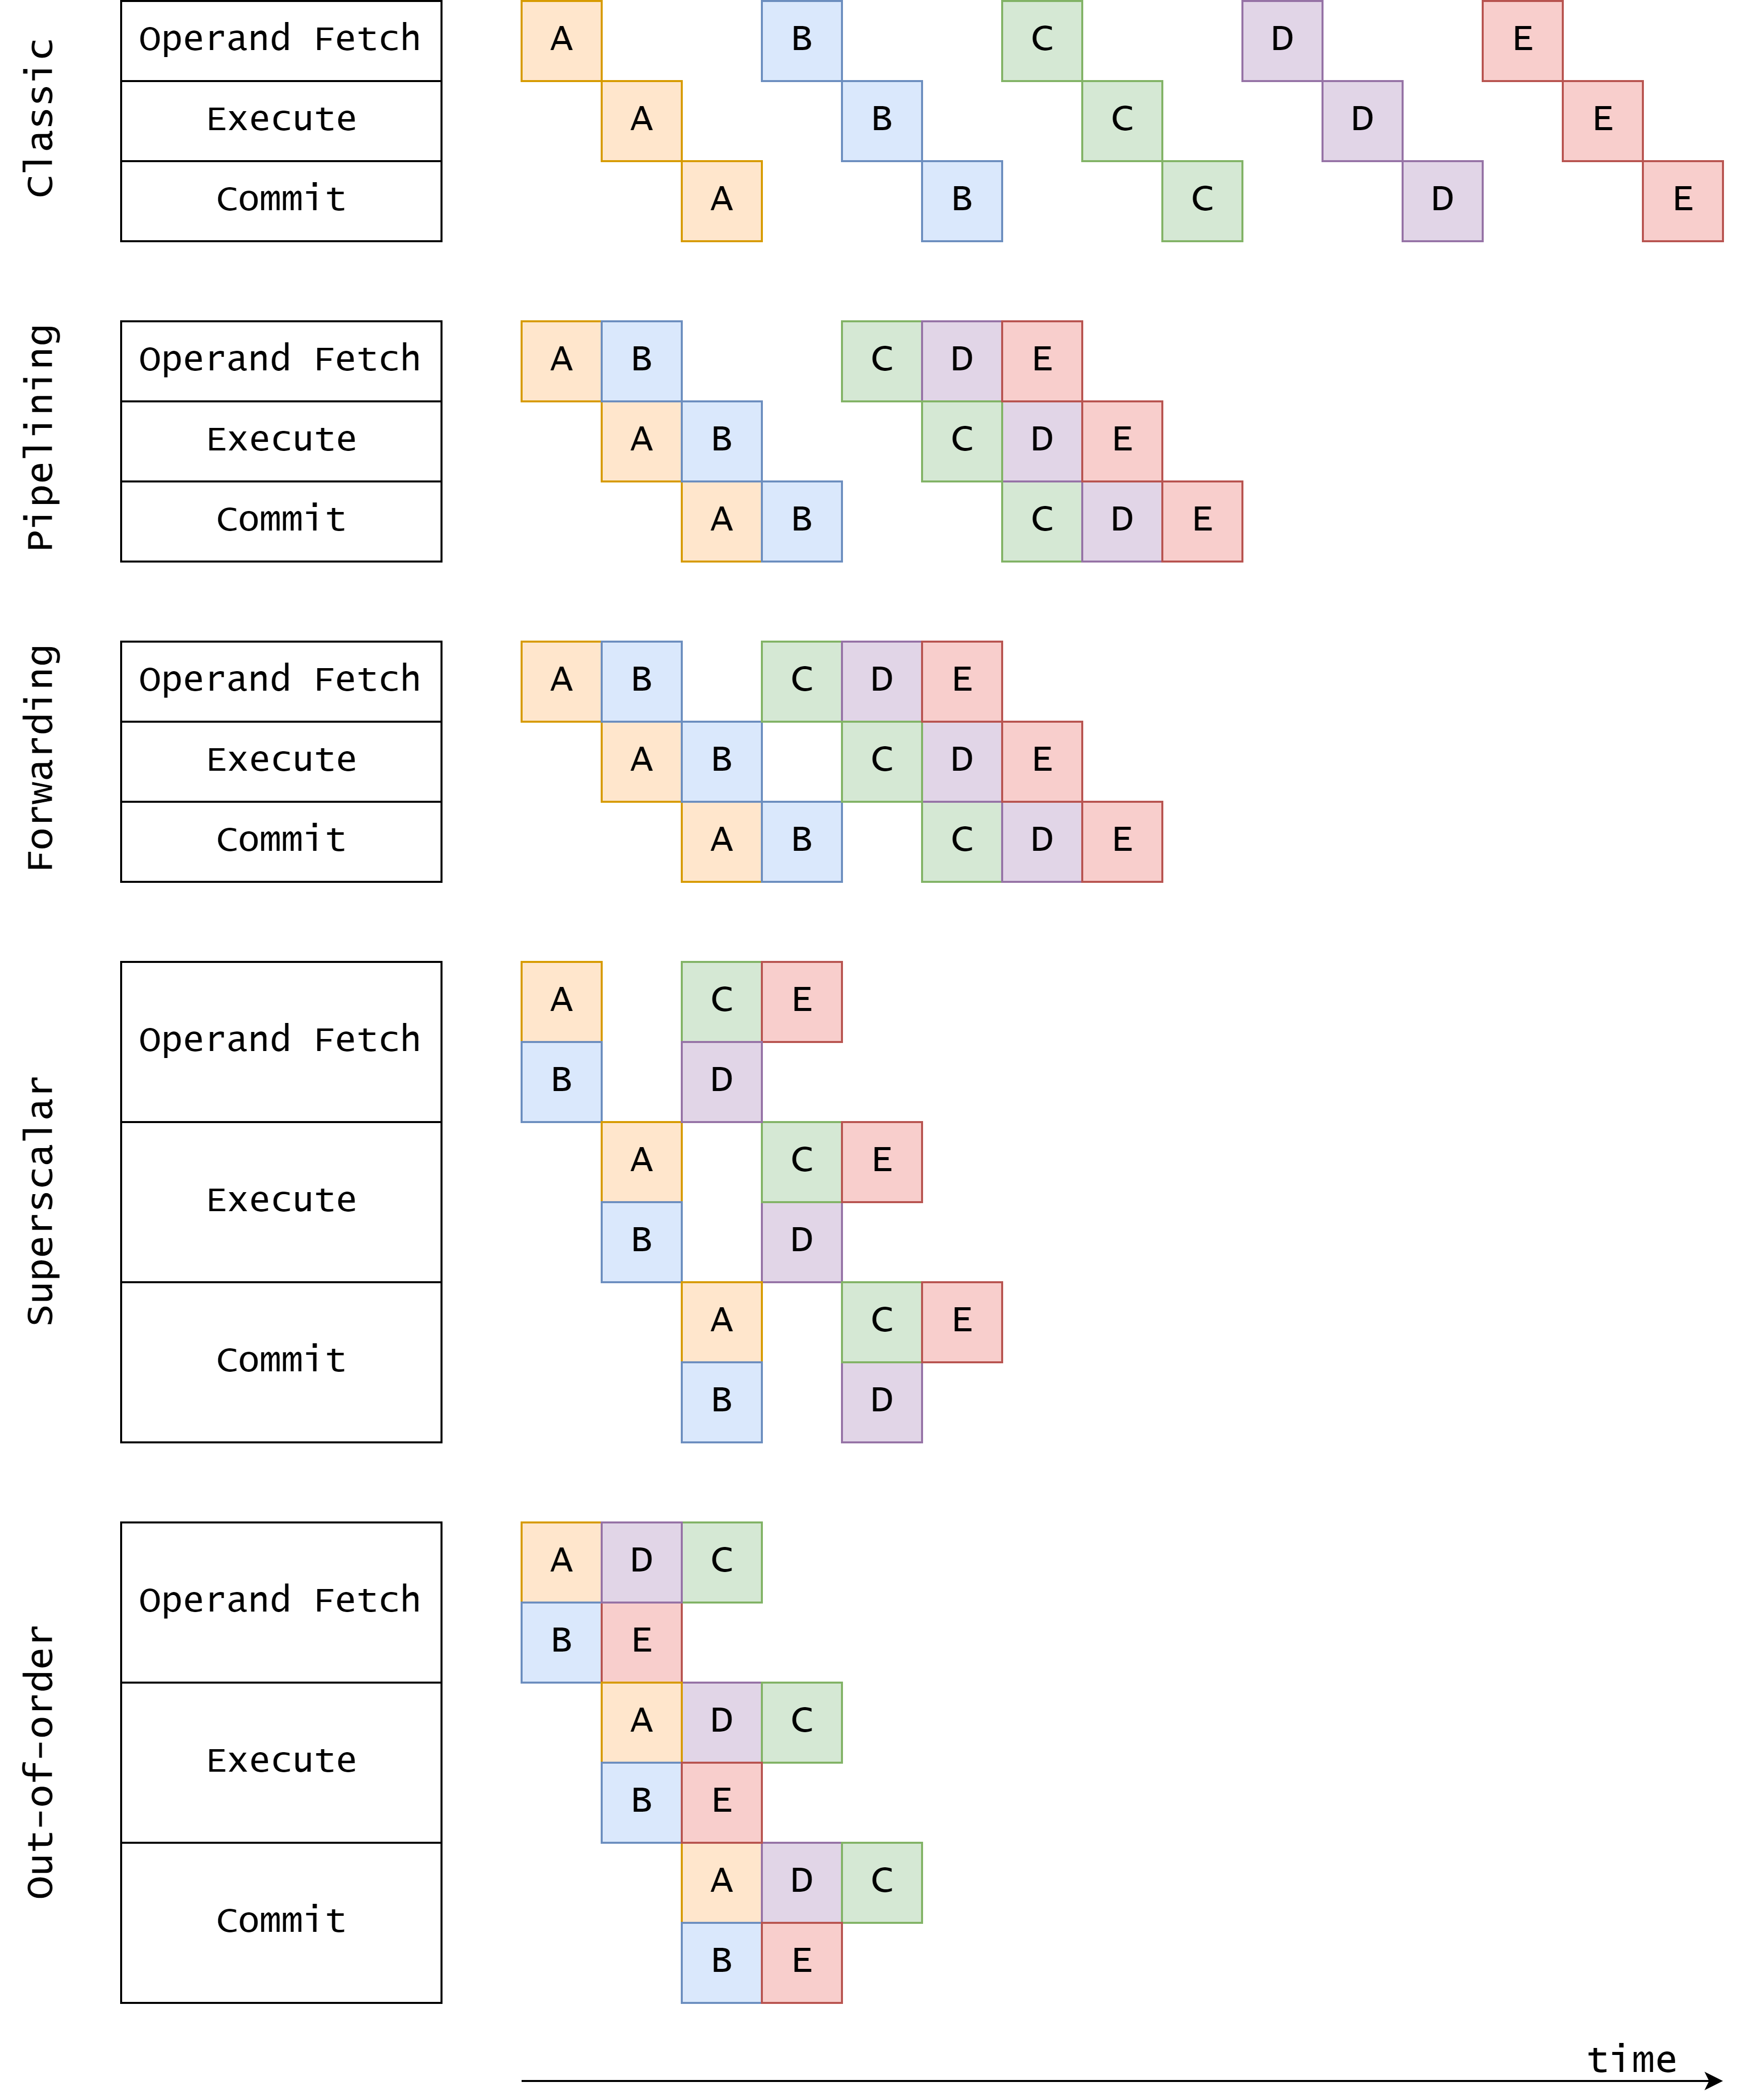
\includegraphics[width=\textwidth]{Source/ExploitingParallelismAlt.png}
	\caption{Overview of the different stages of optimizing a pipeline if there is a data dependency between instructions B\&C.\\
	This assumes that there are enough execution units to simultaneously execute A\&B, C\&D and D\&E, respectively and that all instructions take only one cycle to execute.\\
	For simplicity, this model ignores how instructions are fetched from memory.\\
	\note{Depending on the architecture, different stages may be appropriate. We are also completely ignoring IF and ID. However, these three stages are enough to demonstrate the principles.}} 
	\label{schedulingSchemes}
\end{figure}

\newpage
\section{Design}

\begin{figure}[!h]
	\centering
	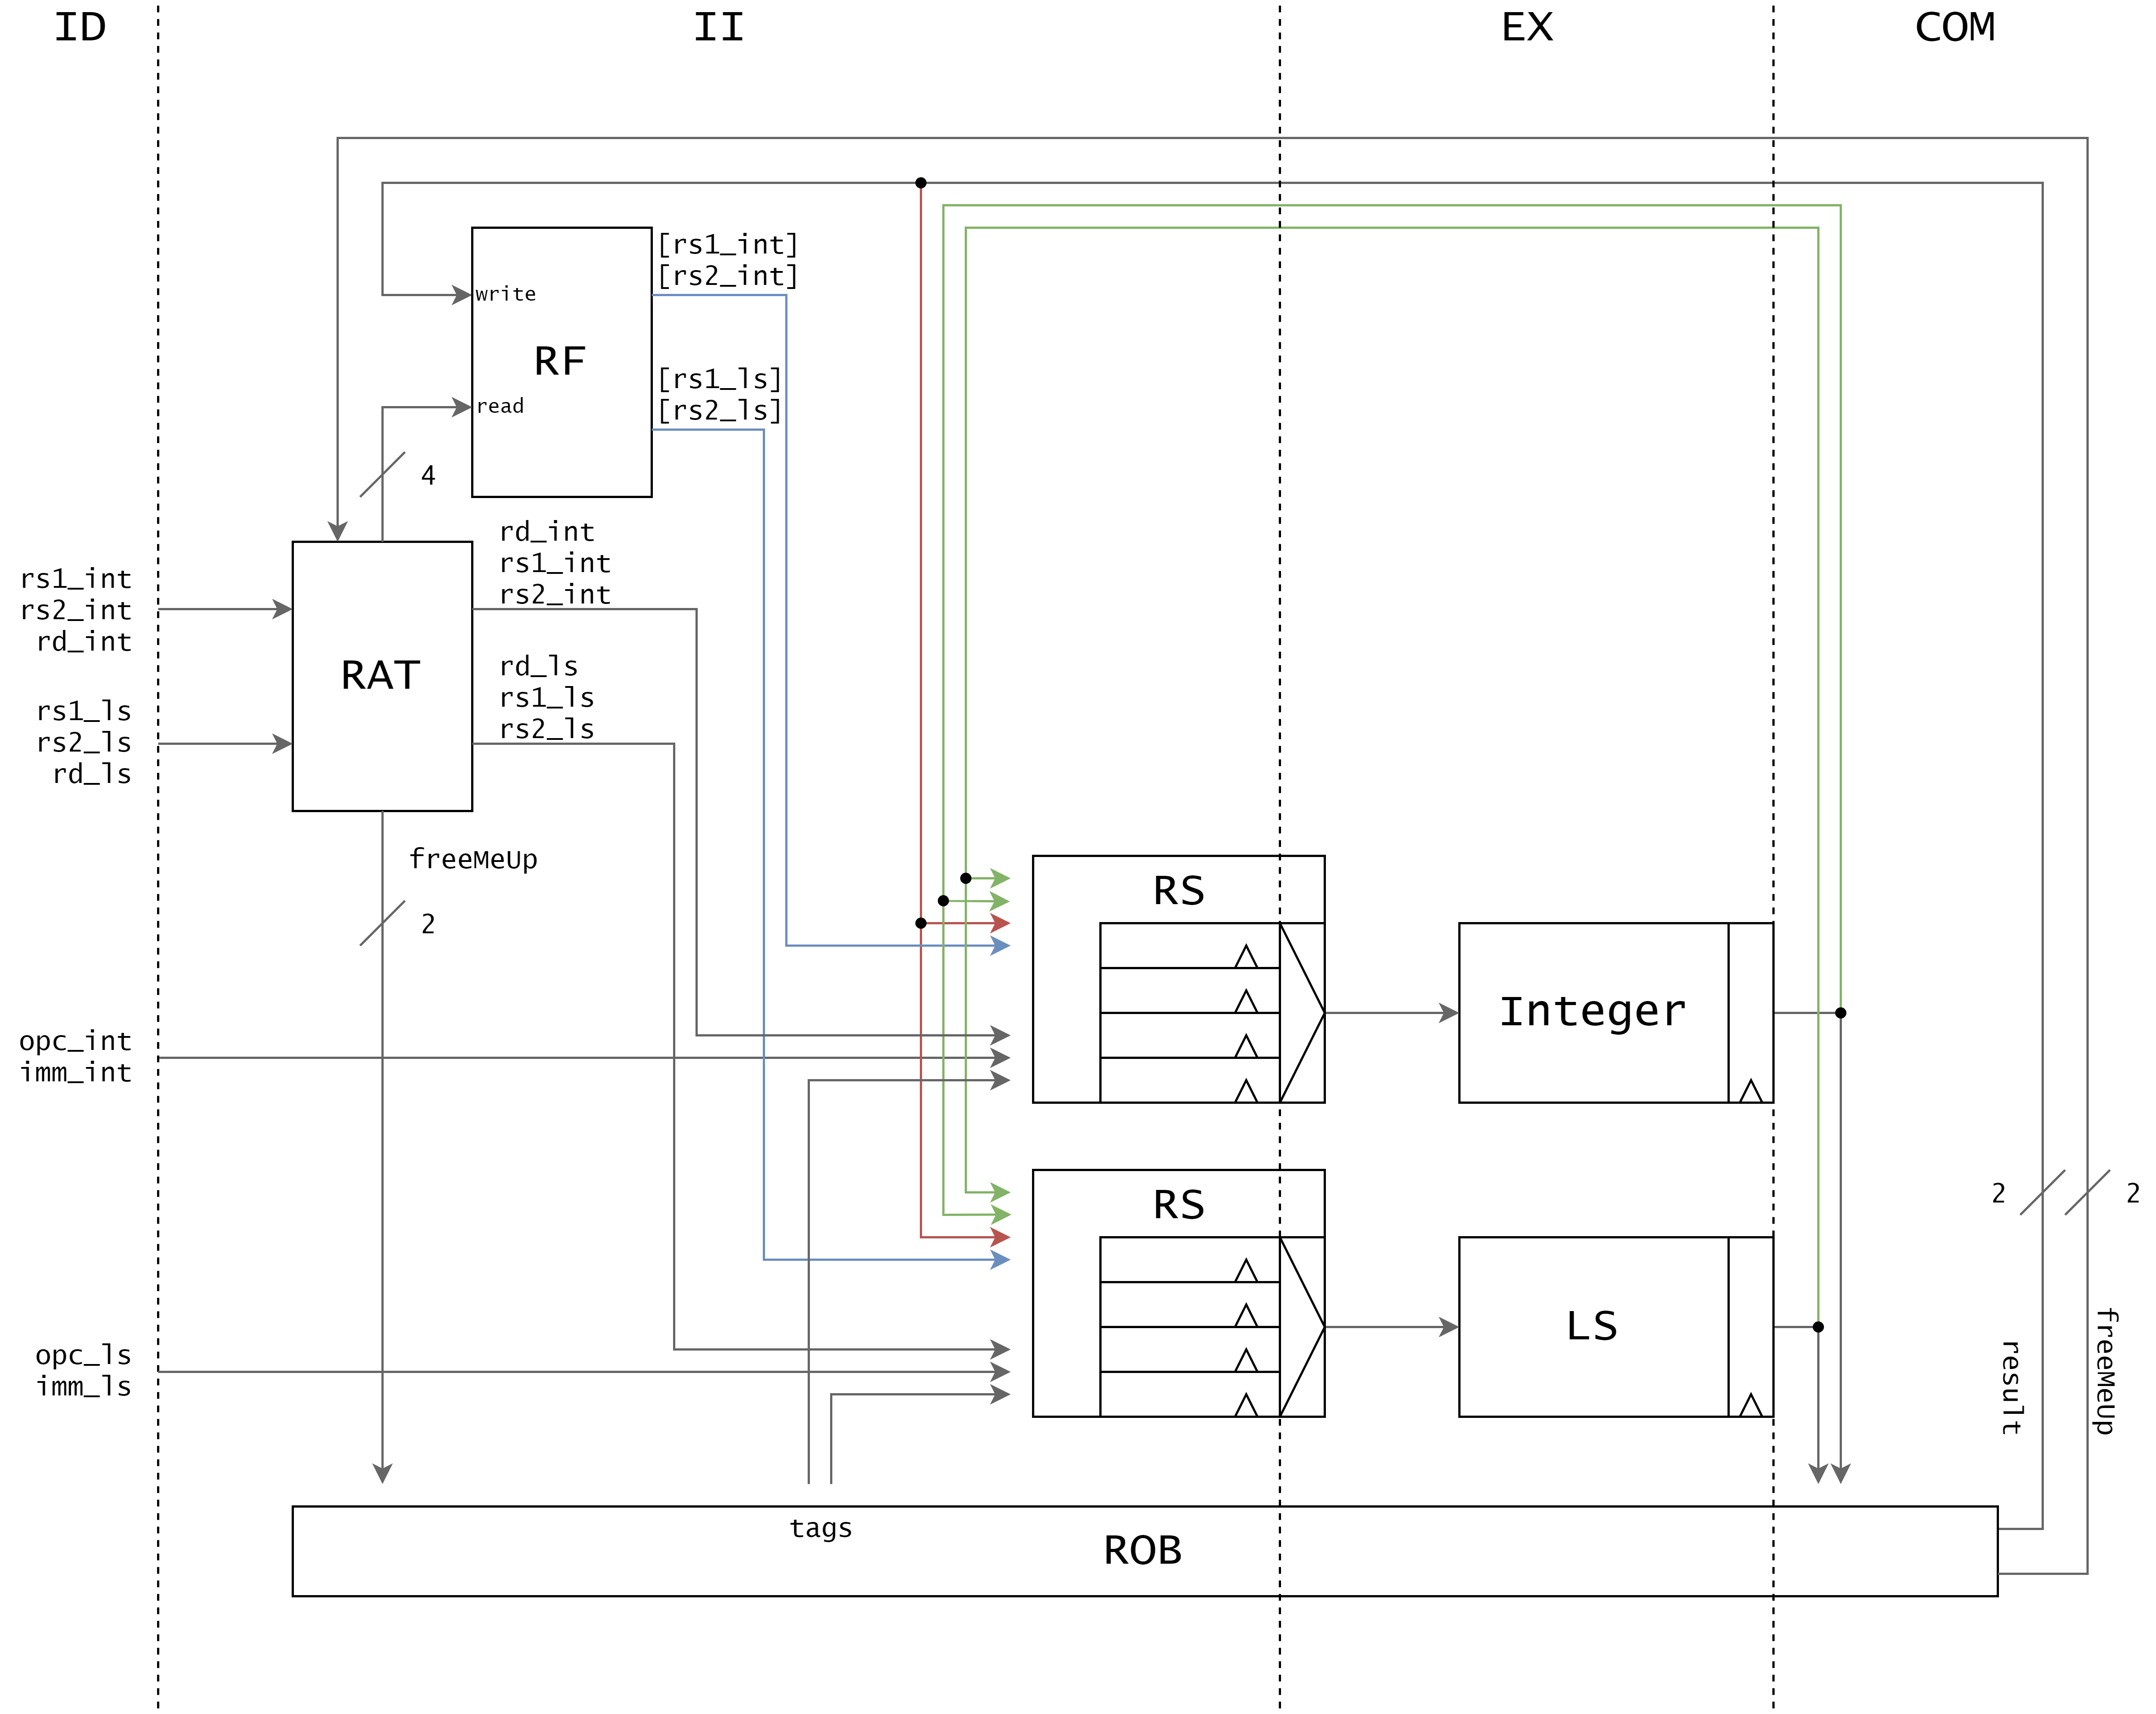
\includegraphics[width = \textwidth]{Source/pipeline.png}
	\caption{Pipeline diagram}
	\label{pipeline}
\end{figure}
Figure \ref{pipeline} shows a high-level diagram of the design that I implemented over the course of this thesis. Let us take a look at the journey of an instruction to understand the different parts.\\
\note{Explain the concept first before explaining every part. It is otherwise really hard to decide on where to put the RF and the ROB}\\
\note{Note that there are different stage naming conventions. Some authors distinguish DISPATCH and ISSUE. COMPLETE, FINISH, RETIRE and COMMIT also are often used interchangeably or used to mean very different things}\\

Every clock cycle the instruction issue stage receives up to two instructions from the decode stage. It tags instructions in program order and renames registers.\\

\note{Maybe have a block diagram of every module?}\\

\subsection{The Register Alias Table (RAT)}
We introduced the idea of register renaming earlier but have not explained how it is implemented. Let us re-examine the example from earlier:
\begin{assembly}
	\begin{tabularx} {\textwidth} {l X}
		ADD & R1, R2, R3\\
		ADD & TODO\\
		ADD & TODO\\
	\end{tabularx}
\end{assembly}

\note{TODO}\\

The register alias table (RAT) keeps track of the mapping between architectural registers and physical registers. In our example above it would look something like this:

\note{TODO Talk about how registers are freed again}

\greyout{
Note that name dependencies can be resolved by register renaming but true dependencies cannot. Consider this example: % We therefore need to be able to detect and distinguish them.\\ 
\begin{assembly}
	\begin{tabularx} {\textwidth} {l X}
		LD  & R1, TODO\\
		LD  & R2, TODO\\	
		ADD & R3, R1, R2\\
	\end{tabularx}
\end{assembly}
The ADD instruction has to wait for both LD instructions to access its source operands. The order of the two load instructions does not matter, however there is no way that the addition can happen first. We may however, execute instructions that come after the addition, while it waits for its operands in so-called reservation stations.
}

\subsection{The Reorder Buffer (ROB)}
The reorder buffer (ROB) tags instructions in program order so that they can \textbf{committed in order} even when their actual execution order is completely different. After instructions are executed, their results are written back to the ROB, where they wait to be committed. \\
The ROB needs to be able to collect as many results and tag and commit as many instructions per cycle as there are execution units to avoid a bottle-neck.

\subsection{The Reservation Stations}
Reservation stations are bundles of registers where instructions wait for their source operands. Every execution unit has their own reservation station. Whenever an execution unit is ready it can start executing any of the instructions in the reservation station that have all their source operands.\\ 
\note{TODO: Explain all the forwarding paths}\\
This prevents instructions from blocking independent instructions that are behind them in program order.

\subsection{The Register File (RF)}
\textbf{Reading the RF}\\
After source and destination registers of an instruction have been renamed, the register file attempts to read the source operands. If they have already been calculated and and written then they can be read, otherwise instructions have to wait for their source operands in so-called reservation stations.\\

\textbf{Writing the RF}\\
The register file is written by the ROB in the commit stage. Register renaming prevents that two consecutive instructions need to write the same register.\\

\textbf{Dimensioning the RF}\\
To implement register renaming effectively, the register file should have more registers than the architectural register file. The base RISC-V ISA specifies 32 (integer) registers. \note{Cite the Specs.} This version uses 64 physical registers, so that it can be addressed with only one bit more. \\
The register file needs to have twice as many read ports as there are execution units, in our case four (two instructions times two source operands). It needs as many write ports as there are execution units, so two here.

\newpage
\section{Results}

\subsection{Superscalarity}
Show that, in theory, this pipeline can have a throughput of 2IPC (if there are no cache misses).
\subsection{Renaming}
Show how destination and source registers are renamed. And show how registers are freed again.
\subsection{Out-of-orderness}
Show how instructions can overtake stalling instructions if they do not depend on them.
\subsection{Limits}
Show an example where due to inherent lack of ILP, the superscalar pipeline shows no advantages

\newpage
\section{Conclusion}
\note{Ideas:}\\

In conclusion, the speed-up from superscalar, out-of-order execution will usually be worth the extra effort and cost.\\
 
In conclusion, we can say that if speed is being prioritised over cost, then a superscalar, out-of-order processor is worth the extra effort. It has become standard in all\\

I have shown one possible implementation of a simple superscalar processor, which demonstrates its major challenges and advantages. 


\newpage
\section{Outlook}
Out of scope:
\begin{itemize}
	\item Control Dependencies (Branches)
	\item Exceptions (maybe quickly explain the difference between precise and imprecise ones) and Interrupts (how to save RF)
	\item How to design the store queue to respect dependencies
	\item Other instructions
	\item SMT
	\item Speculative execution
\end{itemize}

Future work:\\
Further analysis is required to...
\begin{itemize}
	\item Maybe put renaming into the decode stage. Maybe talk about balanced pipelines
	\item Centralized vs distributed reservation stations (\cite[p.202]{lipastiShen} for Pros and Cons)
	\item The perfect mix of execution units is application dependent (\cite[p.205]{lipastiShen})
	\item It can be useful to have more execution units than maximal IPC count because the instruction mix can change a lot across code (\cite[p.206]{lipastiShen})
	\item Alternative way of doing register renaming. Have both a renaming register and an architectural register and shadow it (\cite[p.239]{lipastiShen})
	\item Alternative approach to reservation stations. Use the ROB as reservation stations and for renaming (?)  (\cite[p.259]{lipastiShen})
	\item Alternative: Only forward to the RF. Instructions in the reservation stations read it when both source operands are available  (\cite[p.260]{lipastiShen} data capture) This could reduce forwarding complexity. But we might struggle with read ports in the RF when there are more execution units
	\item Value prediction  (\cite[p.261]{lipastiShen})
\end{itemize}
\note{Reference the appendices}


\newpage
\section{Sort these}

\subsection{Load-Store architecture}
We are working with a load and store architecture, so... \note{explain why it is sufficient to only read registers. Or maybe only talk about that later, when going into details}

\subsection{Dynamic vs static register renaming}
We might wonder why the compiler has to pretend that there are only 32 (architectural) registers, when in reality we have 64. \note{see p.8 physical notes}


\subsection{The anatomy of a RISC-V instruction}
\note{Is this relevant?}

\subsection{The VLIW approach}              
The register renaming and reordering of instructions can be done either at compile time by the compiler (static scheduling) or at execution time by the hardware (dynamic scheduling). The latter can have big advantages because the compiler cannot anticipate all dependencies, as they may rely on external input at execution time. The compiler also cannot anticipate stalls that are caused by unpredictable cache misses, which can cost many clock cycles.\note{we do not need to recompile the same program for every hardware. reference Hennessy}\\

\subsection{History of ILP exploitation}
\begin{itemize}
	\item Pipelining is a form of parallelism
				\begin{itemize}
					\item Started in the 1960s
				\end{itemize}
	\item Power series. Maybe examine the most recent one
				\begin{itemize}
					\item Number of execution units
					\item Number of (renaming) registers
					\item  Number of instructions in flight
				\end{itemize}
	\item Plateau in returns
				\begin{itemize}
					\item Intel Pentium 4
				\end{itemize}
	\item So if we have passed the point of diminishing returns with ILP exploitation (either because the effort is too high or because we actually reach the dataflow limit), what's next?\\
	\note{Hen and Pat claim that we have passed that point in 2005 (see pages 245f) but in table 3.47 we see that issues/clock and number of functional units are still in creasing.So maybe do not use that phrase (passed the point of diminishing returns) but simply say that other techniques have become the focus.\\
	Adapt the table on p.247 (hen and pat) to show that they have focused on increasing caches and the number of cores.}\\
	Maybe talk about data and thread level parallelism.
	\item I am writing this thesis on a ThinkPad with an i7 core. [It has the following specs]\\
	In comparison, [this other computer which came out x years ago] had a similar clock frequency but would still have problems competing with the performance of this ThinkPad. So clock frequency is not everything. \note{Compare architectures}.
	
\end{itemize}

Find sources

\subsection{Other ways to speed up processors}
\begin{itemize}
	\item higher clock rates $\rightarrow$ useful if cooling is no inconvenience
	\item bigger caches
	\item more cores
\end{itemize}

\subsection{Limits to exploitation of ILP}

This is mostly from \url{https://courses.cs.washington.edu/courses/cse471/07sp/lectures/Lecture4.pdfs}

\begin{itemize}
    \item Inherent limit to parallelism in code\\
              Loop unrolling and branch prediction can help\\
              In 1970 Tjaden and Flynn thought that ILP usually is less than 2 (Flynn's bottleneck), but soon later people started realising that if one could circumvent control dependencies, this limit could be much higher. Branch prediction made this possible. Since then many papers working from different assumptions have proposed various ``limits to ILP'' ranging from less than 2 to several dozen. This shows again how application-dependent optimisation can be. \cite[p.25]{lipastiShen}
    \item At some point hardware becomes so complex that the speed-up might be negated
                \begin{itemize}
                    \item Instruction Fetch and Instruction Issue become broader and broader. This can become particularly long if IF has to get more than one Instruction-Cacheline in one cycle.\\
                    Instruction Fetch is limited by misalignment and control dependencies \\
                    Predecoding can help with the ID bottleneck.
                    \item Register File needs many ports
                    \item Both data and instruction caches need more access ports
                    \item Reservation Stations and ROB need to be accessed in parallel
                    \item The complexity of forwarding paths grows both with the number of execution units and the number of execution units
                \end{itemize}
            Maybe make a complexity analysis. If n is the number of execution units and r is the depth of the reservation stations, then the complexity of the rd tag compare for the forwarding paths is $\mathcal(O)(nxr)$ (?).
    \item Plot IPC width against time to show that it has plateaued in the noughties
\end{itemize}


\newpage
\appendix
\section{The physical limits to clock frequency of classical computers or why you cannot buy a laptop with a 10GHz clock rate}
\label{physicallimits}
\note{This should probably not be an appendix. It is starting to become quite a major part...}\\

The average runtime of an instruction is given by
\begin{equation}
\begin{aligned}
\text{Runtime} 
&= \frac{\text{Cycles}}{\text{Instruction}} \times \frac{\text{Time}}{\text{Cycle}}\\
&= \frac{1}{\text{IPC} \times \text{clock rate}} 
\end{aligned}
\end{equation}
where IPC stands for "Instructions per Cycle".\\
\note{I could talk about trade-offs in processor optimisation. (\cite{lipastiShen} p.11ff section 1.3.2) How, increasing IPC can decrease clock rate etc.}\\
Making a processor superscalar is an attempt to reduce runtime by increasing IPC count. However, we can see that it would be just as effective to increase the clock rate. It might seem easier to keep the simple linear pipeline and make our clock twice as fast than to design a complicated pipeline that can handle two instructions at once. Especially now that we have seen how much this increases hardware complexity, we might ask, why do hardware designers bother?\\

To answer this question, this chapter contains several figures plotting various processor characteristics against their release year, mostly taken from the Stanford CPU database \cite{cpudb}. We should note that in recent years it has been becoming harder to account for things like thermal design power, supply voltage and frequency due to dynamic voltage and frequency scaling (DVFS). Intel, for example, offers a turbo mode, configurable TDP (cTDP) and a low-power mode \cite[p.~87-94]{intelDataSheet}. These allow a processor to exceed its standard performance for short amounts of time, or to trade in performance for a longer battery life. Figure \ref{vdd} tried to account for this by plotting a maximum (green) and a minimum (purple) voltage that the manufacturer provided. Such values are unfortunately not always available or representative of the actual average value in real-world applications, especially when it comes to frequency and power \cite{caseAgainstACP}.

\begin{figure}[!h]
	\centering
	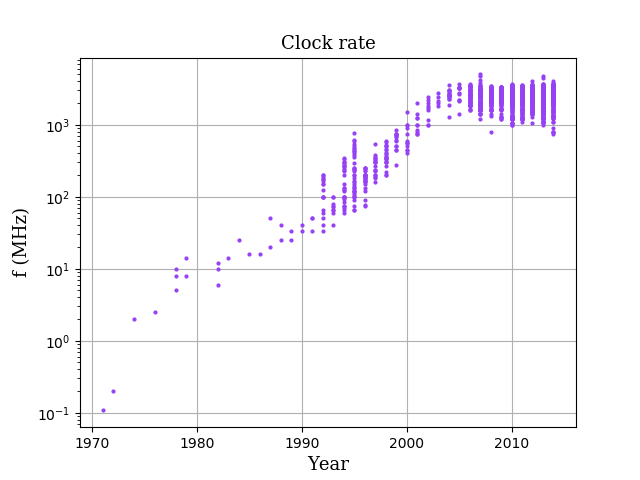
\includegraphics[width=\textwidth]{Source/ClockRate.png}
	\caption{Clock rate over the last 50 years. Drawn with data from \cite{cpudb}} 
	\label{clockrate}
\end{figure}%
Figure \ref{clockrate} shows how clock rate has changed over the last few decades. Up to about 2004, we see an exponential increase (note the logarithmic scale) \note{derive this from Moore's law and Dennard scaling. During this stage it should be correlated with FO4 delay because path delay used to determine clock frequency (\cite{lipastiShen} p.5 top)}, however, since then clock rate has plateaued at around 3GHz.\\


Different authors have different opinions on what has been the major cause for this. \note{Cite at least one for POWER and DELAY}.\\
In this appendix, I want to make the case that power dissipation has been the limiting factor and I want to give an order-of-magnitude explanation of the plateau.\\

\subsection{Power dissipation in CMOS circuits}
First, we need to understand how power consumption scales.
\begin{figure} [h]
	\centering	
    \begin{minipage}{.5\textwidth}
		\centering
		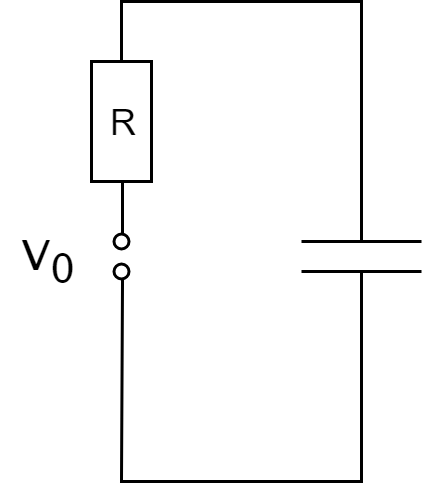
\includegraphics[height = 5cm]{Source/CapacitorCharging.png}
	\end{minipage}%
	\begin{minipage}{0.5\textwidth}
		\centering
		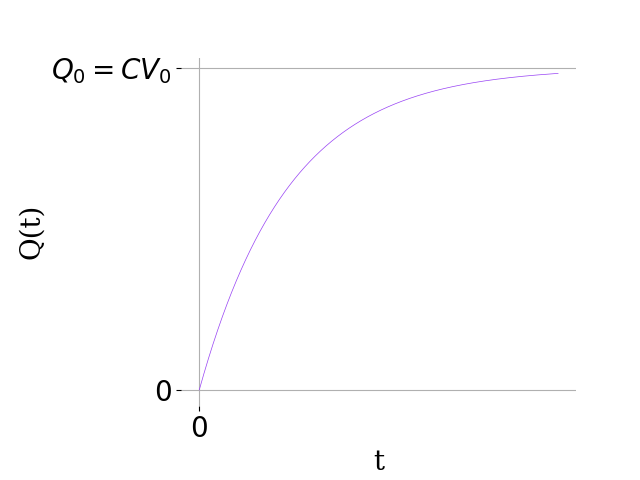
\includegraphics[height = 6cm]{Source/charge.png}
	\end{minipage}
	\caption{Left: R-C charging model. Right: Charge as a function of time for this model }
	\label{capacitorCharging}
\end{figure}

\subsubsection{Dynamic power consumption}
There are two sources of dynamic power consumption in CMOS circuitry. One is switching power, the other is short circuit power.\\

\textbf{Switching power}\\
Power is dissipated wherever parts of the circuitry are being charged/discharged. We can model this as a kind of capacitor which is charged over a resistor which corresponds to the resistance of all the wires and transistors. This is where power is dissipated in the form of heat. Figure \ref{capacitorCharging} illustrates this setup.\\
We are now going to take a closer look at this charging process which is sketched on the right in figure \ref{capacitorCharging}. If we turn on the voltage source at $t=0$, the charge on the capacitor $Q(t)$ will rise to the full $Q_0 = CV_0$, where $V_0$ is the supply voltage and $C$ is the capacity of the capacitor. Figure \ref{capacitorCharging} also shows the current which flows through the resistor. It is simply the derivative of the first curve $I(t)= \frac{d}{dt}Q(t)$. This current determines the how much power is dissipated in the resistor.\\ Every charge transfer $dQ$ onto the capacitor comes with a transfer energy, given by
\begin{equation}
	dE = VdQ
\end{equation}
Capacity $C$ is defined as charge $Q$ per voltage $V$ at any point in time, so we can write this as
\begin{equation}
	dE = \frac{Q}{C} dQ
\end{equation}
For a full charge to $V_0$\footnote{In practice, we will not reach that voltage, however the calculations are similar if we only require a charge of $0.95V_0$.} we find
\begin{equation}
	E = \int_{0}^{Q_0} \frac{Q}{C} dQ = \frac{1}{2} \frac{Q_0^2}{C} = \frac{1}{2} C V_0^2 = \frac{1}{2} Q_0 V_0
\end{equation}
However, the ``battery'' supplies the full $E_{sup} = Q_0 V_0$. So the other $\frac{1}{2}Q_0 V_0$ are dissipated in the resistance in the form of heat. If we also include the heat dissipated in the discharge, then the total energy lost per ``clock cycle'' is
\begin{equation}
	\frac{E}{cycle} = \alpha C V_0^2
\end{equation}
where I have included an activity factor $\alpha$. This accounts for the fact that not every transistor is switching every clock cycle. \note{Maybe make an estimate. Talk about switching activity and dark silicon} \\ 
Now, power is $P=\frac{E}{t}$ and frequency is $f=\frac{cycles}{t}$, so
\begin{equation}
	P = \frac{E}{t} = \frac{E}{cycle} \times \frac{cycles}{t} = \alpha CV_0^2f
\end{equation}
The effective capacitance is given by the feature size and the design of the CPU. Using the Stanford CPU database again, we found this to be around $10^{-8}F$. A similar value was found in \cite{PowerBlogPost}\\
\note{It looks like C has increased a little but mostly stayed the same over the last decades. Maybe find a proportionality argument for this over Moore's law}\\
\begin{figure}[!h]
	\centering
	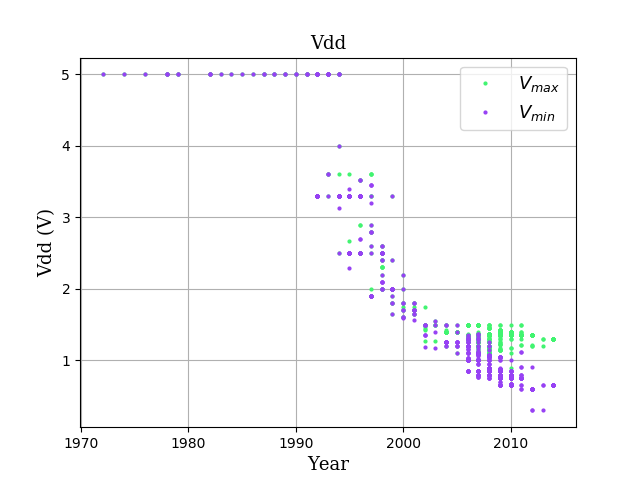
\includegraphics[width=\textwidth]{Source/Vdd.png}%
	\caption{$V_{dd}$ over the last 50 years. Drawn with data from \cite{cpudb}. \note{The extremely low Vdd values are from \url{https://ark.intel.com/content/www/us/en/ark/products/70097/intel-atom-processor-z2480-512k-cache-up-to-2-00-ghz.html}}}%
	\label{vdd}
\end{figure}%
The thermal voltage $\frac{kT}{e} \approx 26mV$ (at $300K$) gives an ultimate lower limit on the operating voltage but there are other factors \note{citation needed} which have resulted in $V_{dd}$ plateauing at around $1V$ (with some manufacturers allowing for lower values in low-power modes).\\
\note{A smaller voltage also means a higher delay (see \cite{LowPowerCMOS}, however this seems to be more of historical interest and is no longer the case)}\\
\note{Also, a higher frequency requires a higher voltage, to preserve correctness, see blog post for experimental proof.}\\
\note{In \cite{ComputingsEnergyProblem} Horowitz claims that voltage scaling has slowed down due to rising leakage currents}\\

This is just working from a very crude model that ignores many things, like that different parts of the CPU have different voltages and frequencies and that not all the parts of the circuitry are active at any point in time. But we can assume that there is some characteristic average value for all these parameters that can be used.\\

\textbf{Short-circuit power}\\
\begin{figure}[!h]
	\centering
	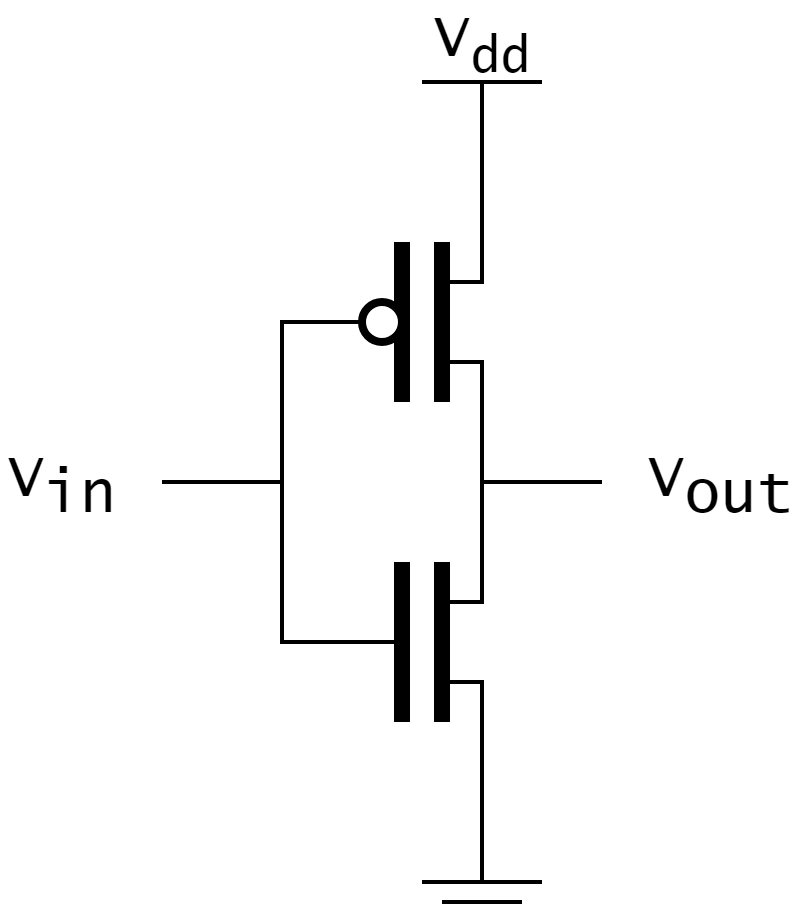
\includegraphics[width=.27\textwidth]{Source/Inverter.png}%
	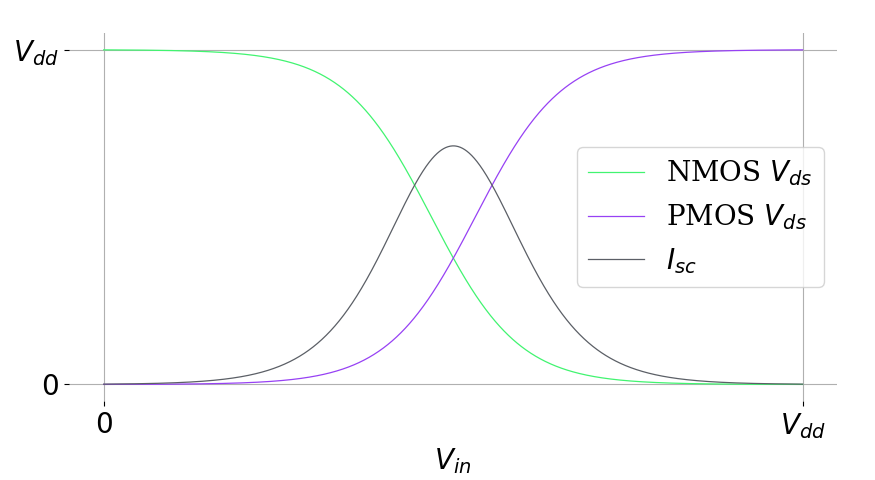
\includegraphics[width=.63\textwidth]{Source/ShortCircuitCurrent.png}%
	\caption{Origin of short-circuit power dissipation (not to scale)}
	\label{Isc}
\end{figure}%
Another source of dynamic power is short-circuit current. The main advantage of CMOS logic over NMOS logic is that, in theory, there is no current path from $V_{dd}$ to $GND$. Consider the inverter in figure \ref{Isc}. Ideally, when $V_{in}$ is high, the nMOS transistor will be on and the pMOS transistor off. The opposite is true when $V_{in}$ is low. Unfortunately, the true behaviour of the MOSFETs is less sharp. When input voltage is switched, there is a time window where both nMOS and pMOS are on, causing a short-circuit.
\note{How much is this? Seems to be negligible, see blog post}\\

Overall, dynamic power scales linearly with frequency.

\subsubsection{Static power consumption}
Sources seem to disagree on whether static power consumption is important or not. Some claim that it is negligible against dynamic power while others have data which seems to prove otherwise. \note{citations needed. see physical notes}.\\

Leakage power \note{TODO}\\ 
\begin{itemize}
	\item Physical source
	\item Temperature dependency
	\item Cadence simulates it as state (process temperature and voltage with k-scaling) dependent and has libraries for that (innovus18.13 - user guide - Innovus User Guide - Analysis Capabilities - Power Analysis and Reports)
\end{itemize}

\note{Static and dynamic power for memory}

\subsection{Cooling limits}
\begin{figure}[!h]
	\centering
	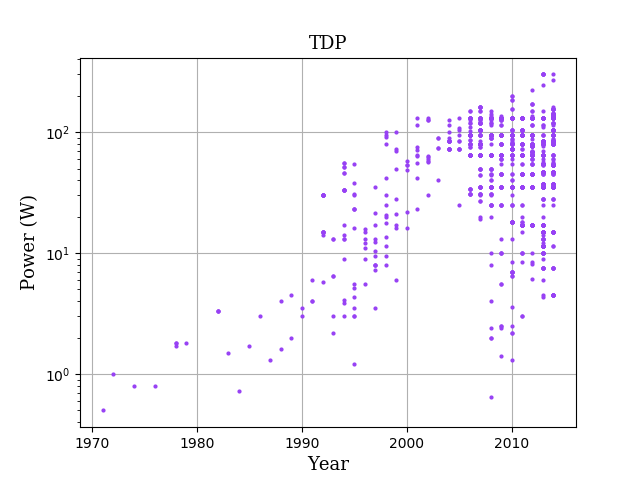
\includegraphics[width=\textwidth]{Source/TDP.png}
	\caption{TDP over the last 50 years. Drawn with data from \cite{cpudb}} 
	\label{tdp}
\end{figure}%
More power means that the system needs to be cooled more. \\
In \cite{ComputingsEnergyProblem}, Horowitz claims that the limit to air cooling for personal computers is around $100W$. Data from the Stanford CPU DB seems to support that estimate. As figure \ref{tdp} demonstrates, the upper limit for thermal design power (TDP) has stagnated at $\approx 200W$ and it did so at around the same time as clock rate (\ref{clockrate}), which further corroborates the claim that it is power limitations that have brought clock frequency to a stall.\\
Figure \ref{tdp} also shows that since then, manufacturers have started offering a wide array of products from low-power to high-power devices. This is an interesting trend of specialisation. \note{TODO. Make clearer what you want to say. Reference the Horowitz paper on specialisation as a counter to the energy problem \cite{ComputingsEnergyProblem} and \cite{ApplicationDependentScaling}, \cite{MaintainingBenefitsWhenScalingBogsDown} and \cite{PowerConstrainedCMOSScalingLimits}, which all say that application-specific optimisation has allowed us and will continue to allow us to scale performance.}




\vspace{2cm}



\note{Note that we are also completely ignoring memory. Both as a source of delay and as a source of static and dynamic power consumption}

\vspace{2cm}
\subsection{Gate and transmission delay}
The telegrapher's equation:

\note{TODO: RC delay model}\\

\note{TODO: LC regime interconnects via modulation \cite{LCSpeedOfLightInterconnects}}\\

\note{TODO: Optical interconnects.\\
	Pros: Speed of light \\
	Contras: expensive, conversion method needed that adds delay ``transformation overhead''}\\

Estimate for transmission delay: $v = 10^{8}\frac{m}{s}$
\begin{equation}
f = \frac{1}{T} = \frac{v}{x} = 
\begin{cases}
	10^{10}Hz \quad \text{for x = 1cm}\\
	10^{11}Hz \quad \text{for x = 1mm}\\
	10^{17}Hz \quad \text{for x = 1nm}\\
\end{cases}
\end{equation}
Transmission delay is not going to limit clock speeds in the near future, as long as wire paths do not get convoluted enough to exceed a centimetre. \\

Could gate delay be the limiting factor?
The FO4 metric can be

\note{TODO: Memory access as a limiting factor? Only if we insist that first-level cache access is one clock cycle}\\

This estimation explains why we have seen a plateau in clock speed over the last decade. Higher clock speeds will require a more sophisticated cooling method or transistor design.

\subsection{Alternative approaches to computing}
These limits could also potentially be overcome by pursuing more exotic approaches to computing, like asynchronous or neuromorphic logic. However, the investment barrier might be to high for such radical changes. In \cite{ComputingsEnergyProblem} Horowitz states that he is ``sure there are better technologies out there'' but that we might be stuck with CMOS for computing because of two big reasons. Firstly, we have invested enormously in the physical manufacturing process of CMOS technologies and any competition would have to have a huge inherent advantage to compete with it. Secondly, CMOS VLSI has greatly influenced our design abstractions. A new technology would require a completely new design flow and new tools to compete. \note{Maybe come up with a CMOS design abstraction that does not translate to for example neuromorphic logic.}\\
Single-core performance is still rising, even though clock speeds have stagnated \note{citation needed $\rightarrow$ Spec INT 2006}. But when it eventually reaches its limits and all inherent parallelism is exploited, other technologies might have a chance to shine. Until then, researchers looking into things neuromorphic, asynchronous or quantum logic need to develop tools and design abstractions to make their technologies viable alternatives.

\greyout{
\subsection{Alternative approaches to computing}
This chapter explores if there are other computing approaches that do not have the power problem presented above. \\
\note{neuromorphic computing, quantum computing, asynchronous computing?}
\subsection{More exotic bounds to computing}
\note{Seth Lloyd. Off topic?}
}

\newpage
\label{meltdown}
\section{Meltdown and Spectre: The dangers of out-of-order speculative execution}
\note{The underlying reason for these exploits is the difference between the architectural state of the processor and the micro-architectural (physical) state.}\\

\note{Maybe put this into the Outlook chapter}

\newpage 
\thispagestyle{empty}
\begin{thebibliography}{56}    
    
    % Uses the MLA style
    
    \bibitem{cpudb}
    Stanford VLSI Group, CPU DB, \url{cpudb.stanford.edu}, accessed 20.04.2019.   
    
    \bibitem{Hennessy}
    Hennessy, John L., and Patterson, David A.. \textit{Computer architecture: a quantitative approach}. Elsevier, 2011.
    
    %\bibitem{DennardScaling}
    %Frank, David J., et al. ``Device scaling limits of Si MOSFETs and their application dependencies." \textit{Proceedings of the IEEE} 89.3 (2001): 259-288.
    
	\bibitem{lloydLimits}
	Lloyd, Seth. ``Ultimate physical limits to computation.'' Nature 406.6799 (2000): 1047.
    
    \bibitem{PowerBlogPost}
    Wong, Henry. ``A Comparison of Intel’s 32nm and 22nm Core i5 CPUs: Power, Voltage, Temperature, and Frequency'' (2012)\\ \url{blog.stuffedcow.net/2012/10/intel32nm-22nm-core-i5-comparison}

	\bibitem{LCSpeedOfLightInterconnects}
	Chang, Richard T., et al. ``Near speed-of-light signaling over on-chip electrical interconnects.'' IEEE Journal of Solid-State Circuits 38.5 (2003): 834-838.
	
	\bibitem{ComputingsEnergyProblem}
	Horowitz, Mark. ``Computing's energy problem (and what we can do about it).'' 2014 IEEE international solid-state circuits conference digest of technical papers (ISSCC). IEEE, 2014.
    
    \bibitem{LowPowerCMOS}
    Chandrakasan, Anantha P., Samuel Sheng, and Robert W. Brodersen. ``Low-power CMOS digital design.'' IEICE Transactions on Electronics 75.4 (1992): 371-382.
    
    \bibitem{ApplicationDependentScaling}
    Frank, David J., et al. ``Device scaling limits of Si MOSFETs and their application dependencies.'' Proceedings of the IEEE 89.3 (2001): 259-288.
    
    \bibitem{MaintainingBenefitsWhenScalingBogsDown}
    Nowak, Edward J. ``Maintaining the benefits of CMOS scaling when scaling bogs down.'' IBM Journal of Research and Development 46.2.3 (2002): 169-180.
    
    \bibitem{PowerConstrainedCMOSScalingLimits}
    Frank, David J. ``Power-constrained CMOS scaling limits.'' IBM Journal of Research and Development 46.2.3 (2002): 235-244.
    
    \bibitem{intelDataSheet}
    Intel Corporation, ``8th and 9th Generation Intel® Core™ Processor Families Datasheet.'', Volume 1 of 2, Revision 003 (2019).
    
    \bibitem{caseAgainstACP}
    Huck, Scott. "Measuring processor power." Intel Corporation (2011).
    
    \bibitem{lipastiShen}
    Shen, John Paul, and Mikko H. Lipasti. Modern processor design: fundamentals of superscalar processors. Waveland Press, 2013.
\end{thebibliography}

\newpage
\thispagestyle{empty}

\textbf{Erklärung}\\

Ich versichere, dass ich diese Arbeit selbstständig verfasst und keine anderen als die angegebenen Quellen und Hilfsmittel benutzt habe.\\

Heidelberg, den \\ %TODO

\vspace{2cm}
Amanda Matthes

\end{document}